\section{Results}\label{sec:results}


I compute the dynamic aggregation of the average treatment effect on the treated group for the least and most supporting precincts and display the results in Table~\ref{tab:att_comparison_combined}.
Also shown are the estimate's standard errors, confidence intervals, and Wald-test p-values for the pre-test of the parallel trends assumption.
Both estimated ATTs are not statistically significant for the close election design.
Furthermore, the least supporting precinct's ATT is not especially economically significant. 
Half a percent of the menu program's budget is roughly \$7,500. 
That is not even enough to afford two speed humps.

Additionally concerning are the extremely low p-values for the pre-trends test.
This test indicates that the close election design likely does not guarantee that parallel trends hold.
This failure may be because factors influencing the trend of infrastructure spending and needs correlate with the election outcome.
Alternatively, it could be because the margin chosen is too large to ensure that the two groups are similar.
The results of the competitive elections design are susceptible to the number of precincts included, often changing the sign of both estimated ATTs.
Note that the treatment effect for the least supporting precincts is over five times larger than the treatment effect estimated in the competitive election design.
Table~\ref{tab:att_comparison_combined} shows a much larger Wald-test p-value for the pre-trends test.
These values indicate that perhaps the indictment design's assumption is more believable than the close election design's assumption.
However, I also see that the most supporting precinct's treatment effect, while statistically significant, is similar in magnitude to the treatment effect of the competitive election design.

\begin{table}[H]
    \centering
    \caption{Comparison of average treatment effects}
    \label{tab:att_comparison_combined}
    \begin{tabular}{lcc|cc}
    \hline
     & \multicolumn{2}{c|}{Competitive Election} & \multicolumn{2}{c}{Indictment} \\
     & Opposing ATT & Supporting ATT & Opposing ATT & Supporting ATT \\
    \hline
    ATT & 0.50 (0.45) & -1.51 (1.12) & 2.59 (0.78) & -1.15 (0.32) \\
    95\% Conf. Int. & (-0.38, 1.39) & (-3.71, 0.68) & (1.06, 4.11) & (-1.77, -0.52) \\
    Pre-Trends P-value & 0.005  & 0.076 & 0.199 & 0.174 \\
    Observations & 1680 & 1680 & 1144 & 1144 \\
    \hline
    \end{tabular}
\end{table}

Figure~\ref{fig:ATT_over_time} depicts how the four designs estimated ATTs vary over time.
All designs except for Panel~\ref{fig:ATT_over_time:corruption_top} passed a placebo test for the last several years before the first treatment.
Panel~\ref{fig:ATT_over_time:corruption_top} shows evidence of anticipation in the year before the first treatment, as the 2019 estimate is significantly smaller than the other estimates.
As inferred from the standard errors in Table~\ref{tab:att_comparison_combined}, the estimated effect over time is noisy for all four designs.
The large noise is likely because even a benevolent social planner will not allocate infrastructure spending using a highly auto-correlated spending rule.
A road, once paved, does not need to be repaved for approximately 20 years, according to CDOT's life cycle analysis \citep{OIGaudit}.
There is a limit to how much spending can be preferentially allocated to a precinct before that alderman runs into harshly diminishing returns.
Despite this, Panels~\ref{fig:ATT_over_time:corruption_bottom} and~\ref{fig:ATT_over_time:corruption_top} both show statistically significant effects post-treatment.
The standard errors, while large, are much smaller for these panels, and the mean estimate is much more stable.
This pattern also holds for the most supporting precincts, albeit in reverse.
Thus, as the incumbent alderman leaves office, they allocate more spending to their most supporting precincts than their least supporting precincts.
Therefore, the gap found must be taken with a grain of salt due to the high standard errors and the likely pre-trends violation.

\begin{figure}[H]
    \centering
    \caption{ATT over time for the four designs}
    \label{fig:ATT_over_time}

    % First row
    \begin{subfigure}{.48\linewidth}
        \centering
        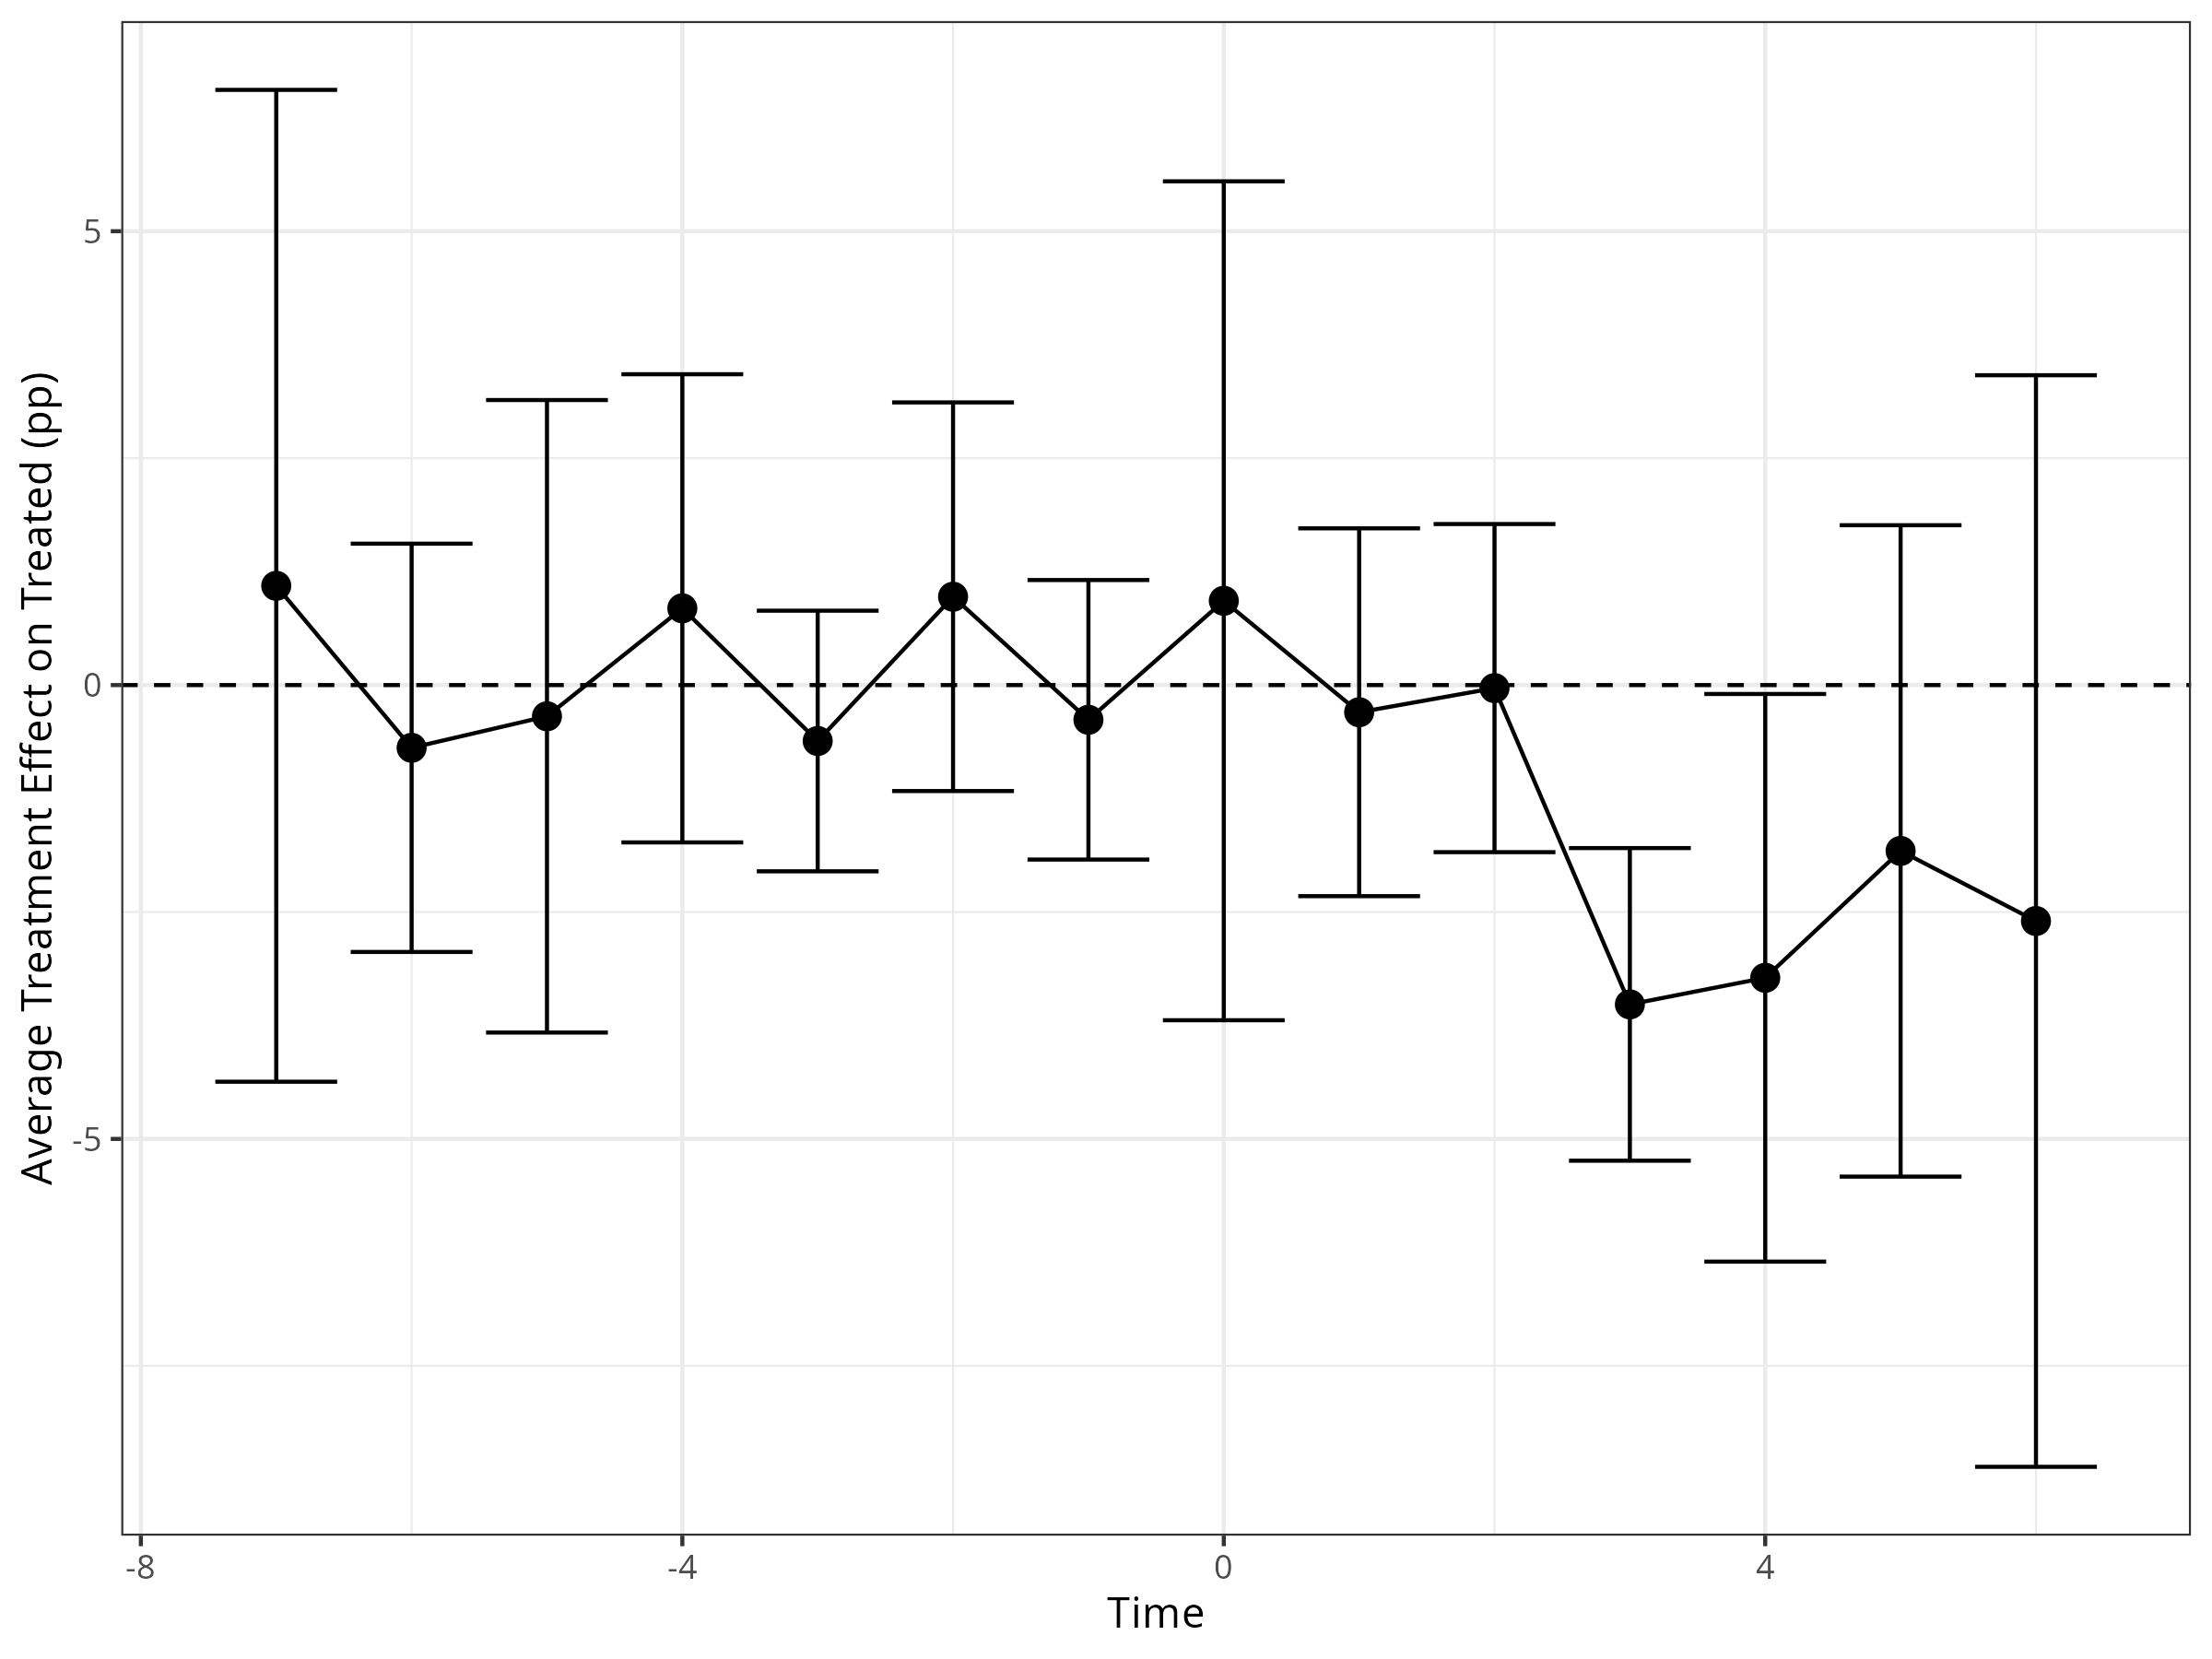
\includegraphics[width=\linewidth]{input/close_elections_8_top_over_time.png}
        \caption{Close Election: most supporting precincts}
        \label{fig:ATT_over_time:close_election_top}
    \end{subfigure}\hfill
    \begin{subfigure}{.48\linewidth}
        \centering
        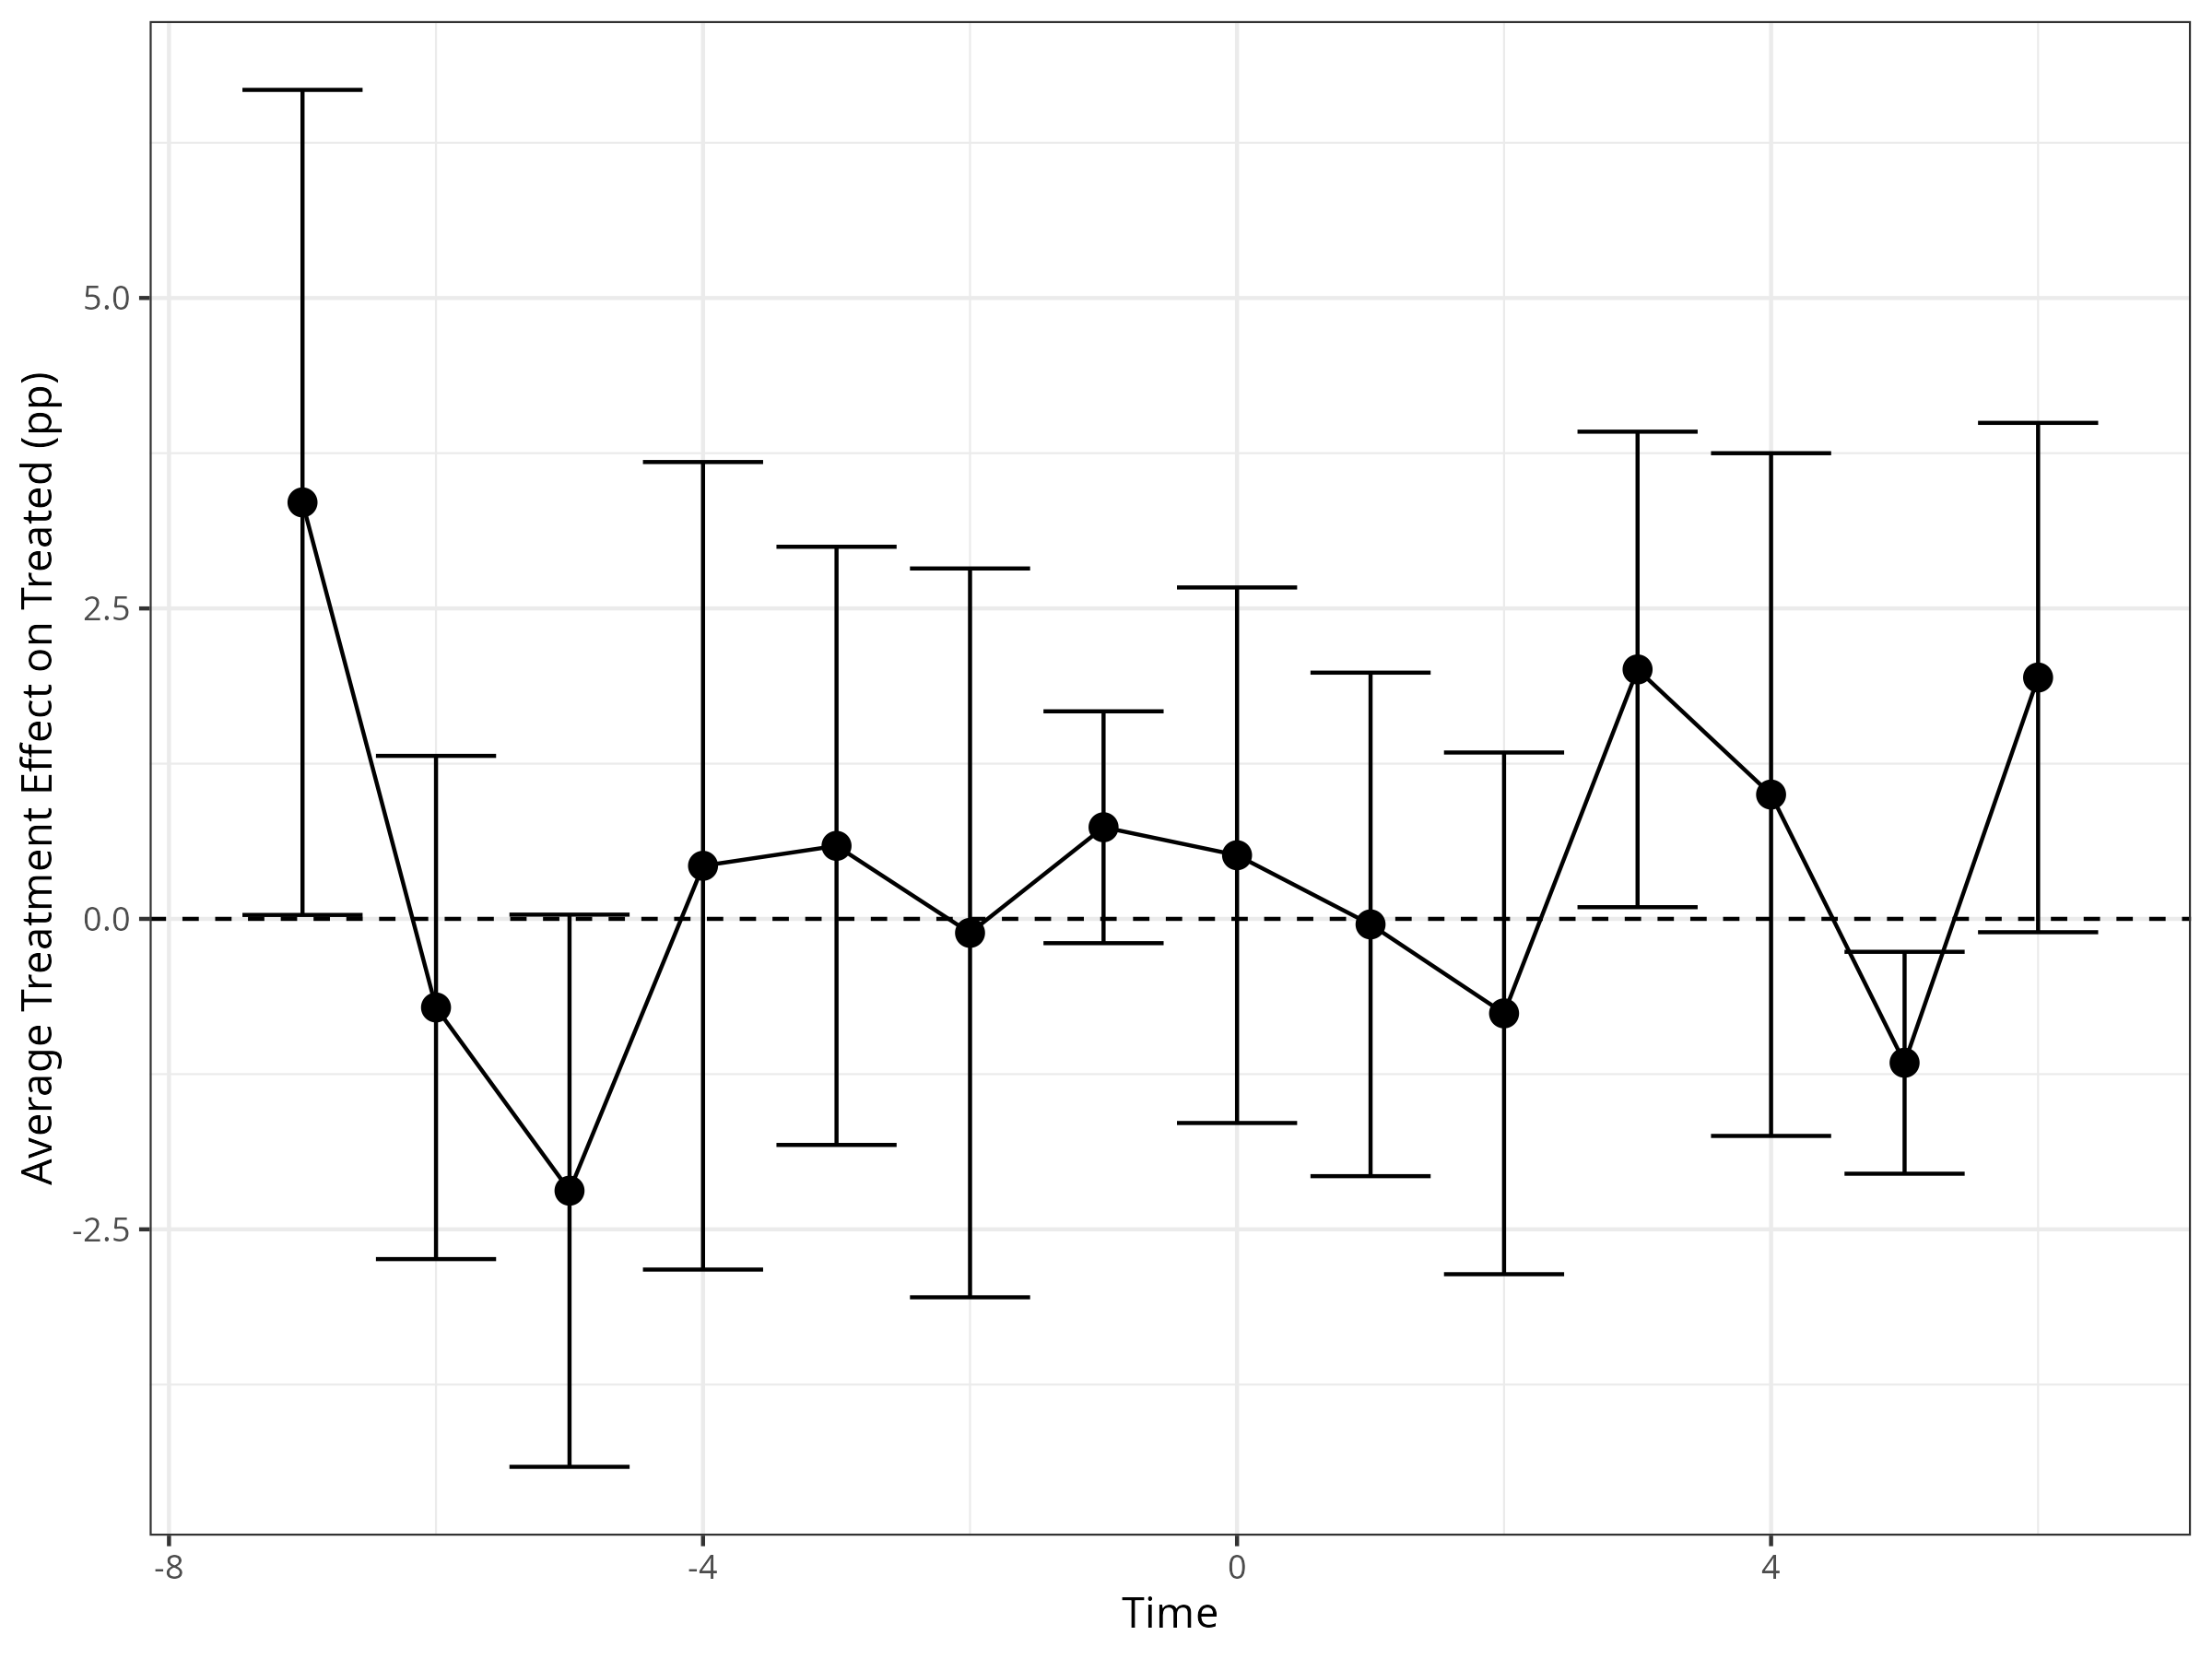
\includegraphics[width=\linewidth]{input/close_elections_8_bottom_over_time.png}
        \caption{Close Election: least supporting precincts}
        \label{fig:ATT_over_time:close_election_bottom}
    \end{subfigure}

    % Second row
    \begin{subfigure}{.48\linewidth}
        \centering
        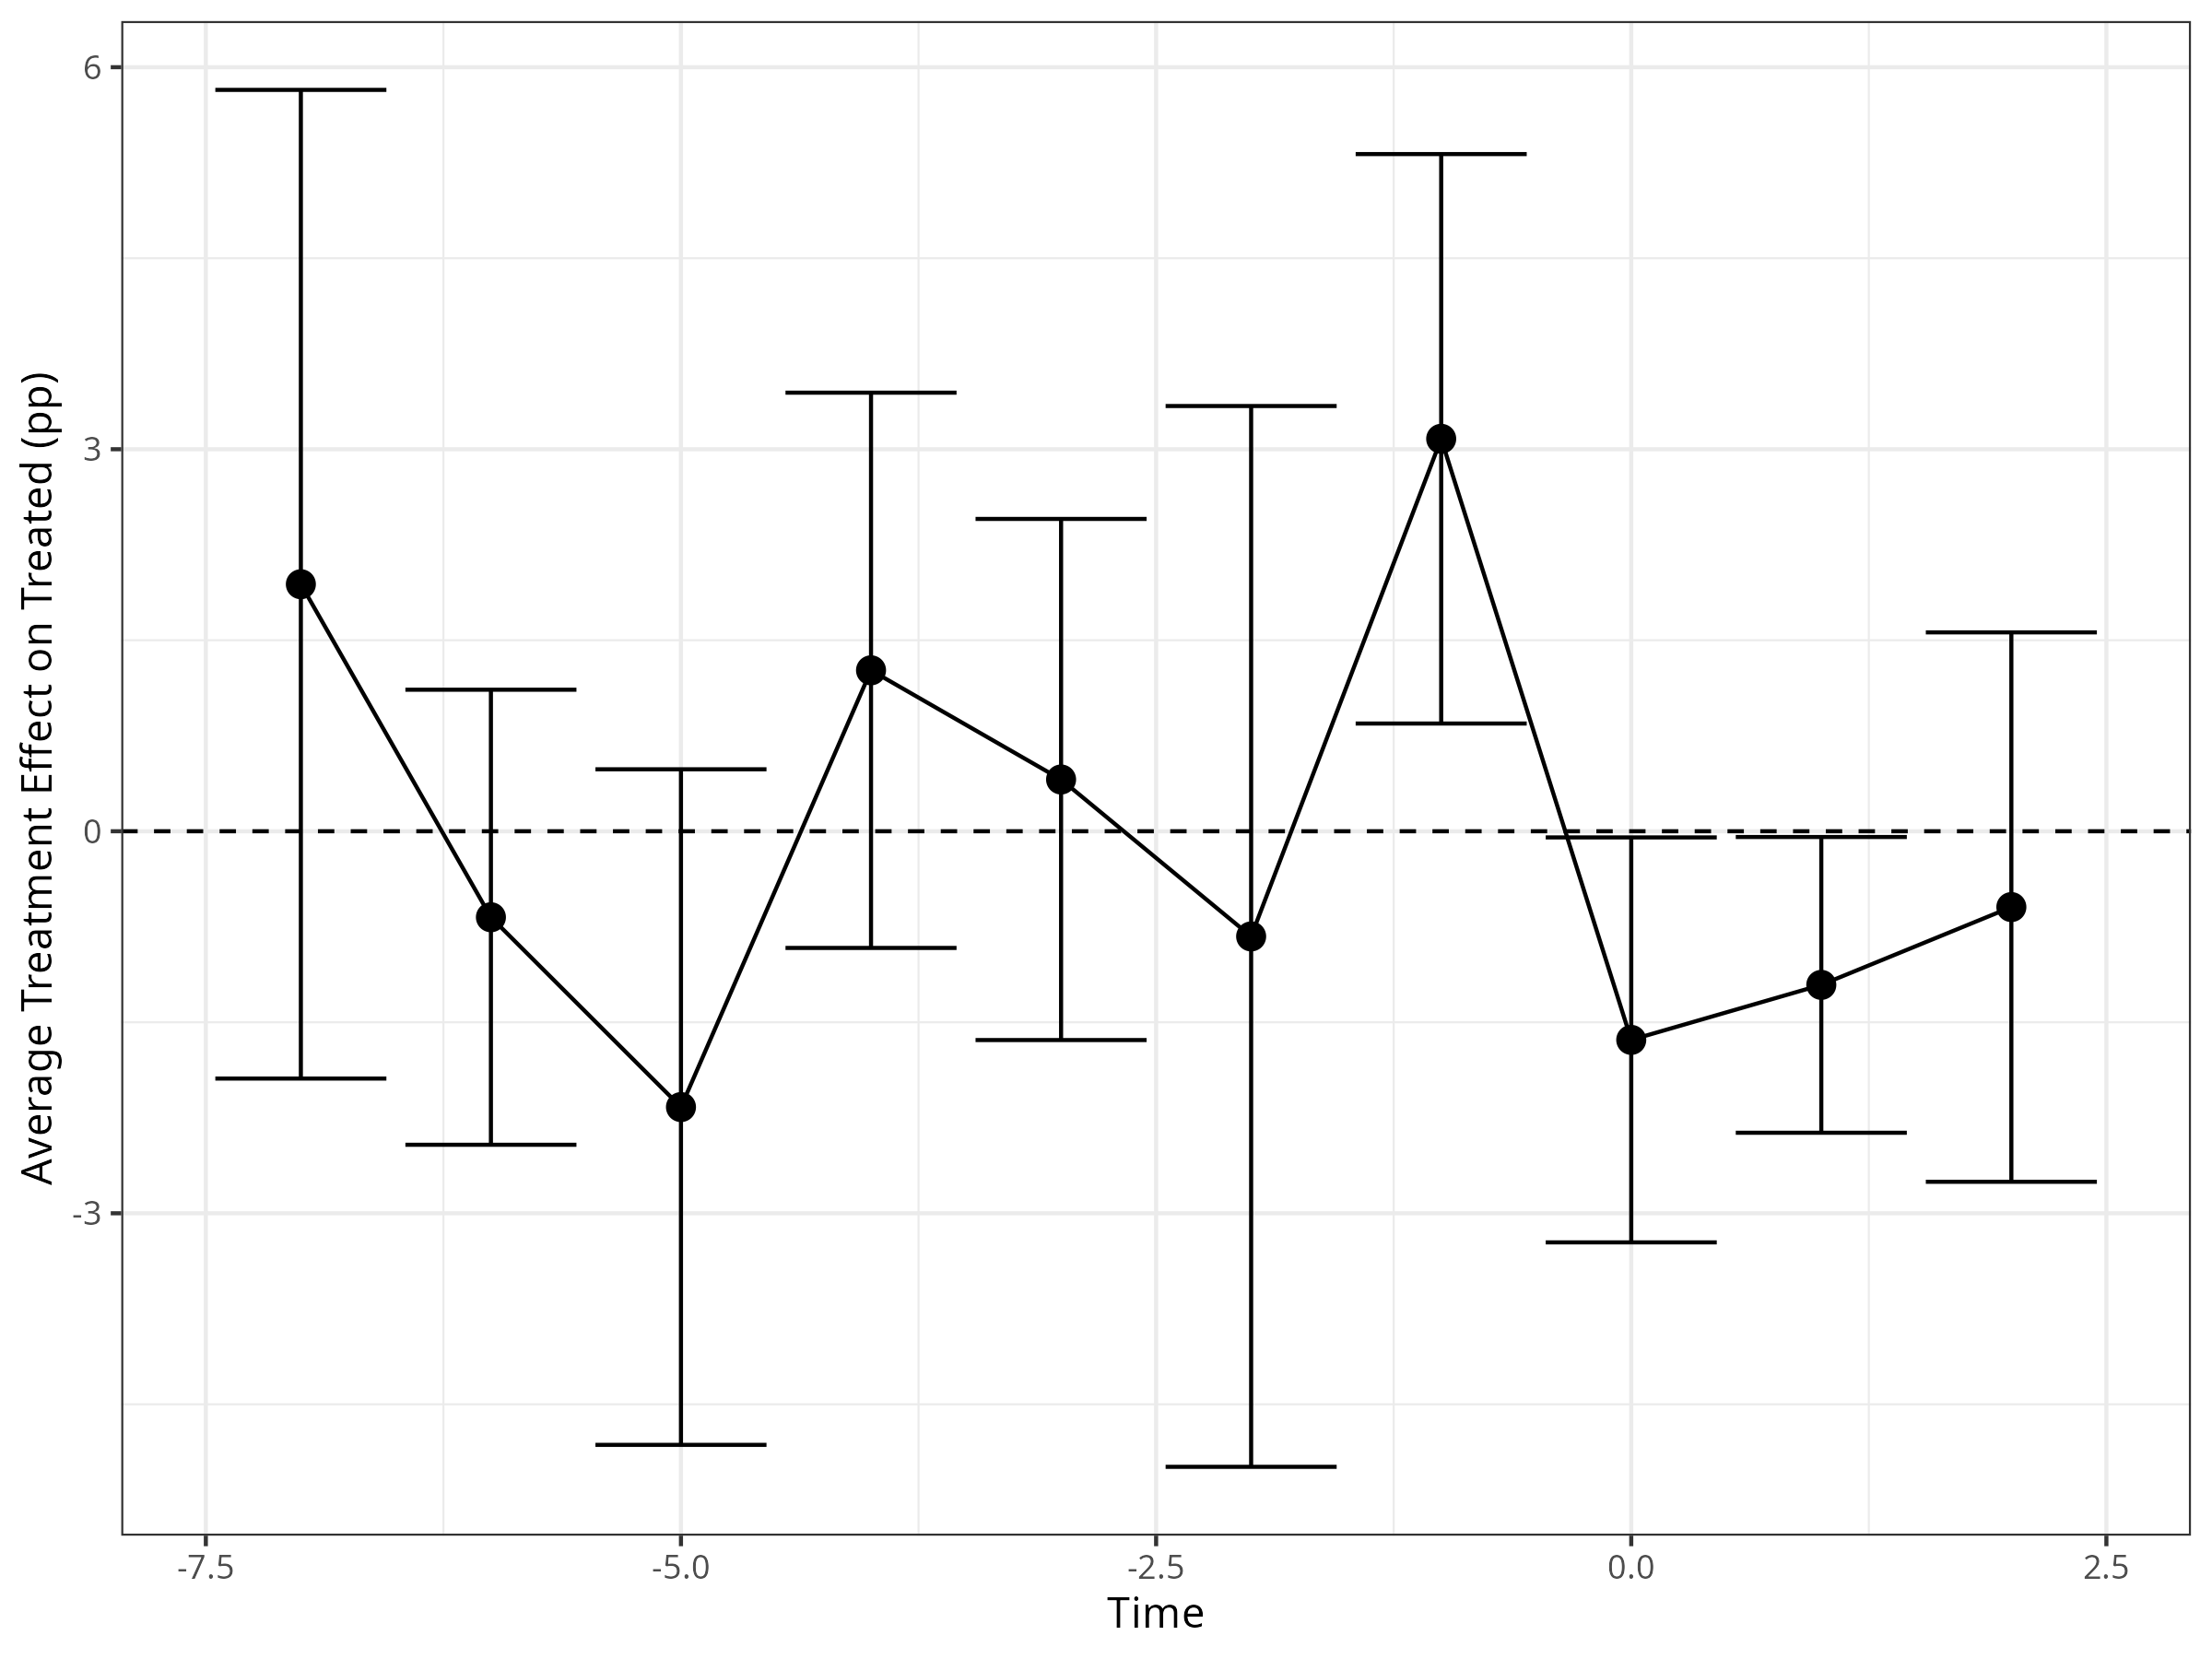
\includegraphics[width=\linewidth]{input/corrupt_8_top_over_time.png}
        \caption{Corruption: most supporting precincts}
        \label{fig:ATT_over_time:corruption_bottom}
    \end{subfigure}\hfill
    \begin{subfigure}{.48\linewidth}
        \centering
        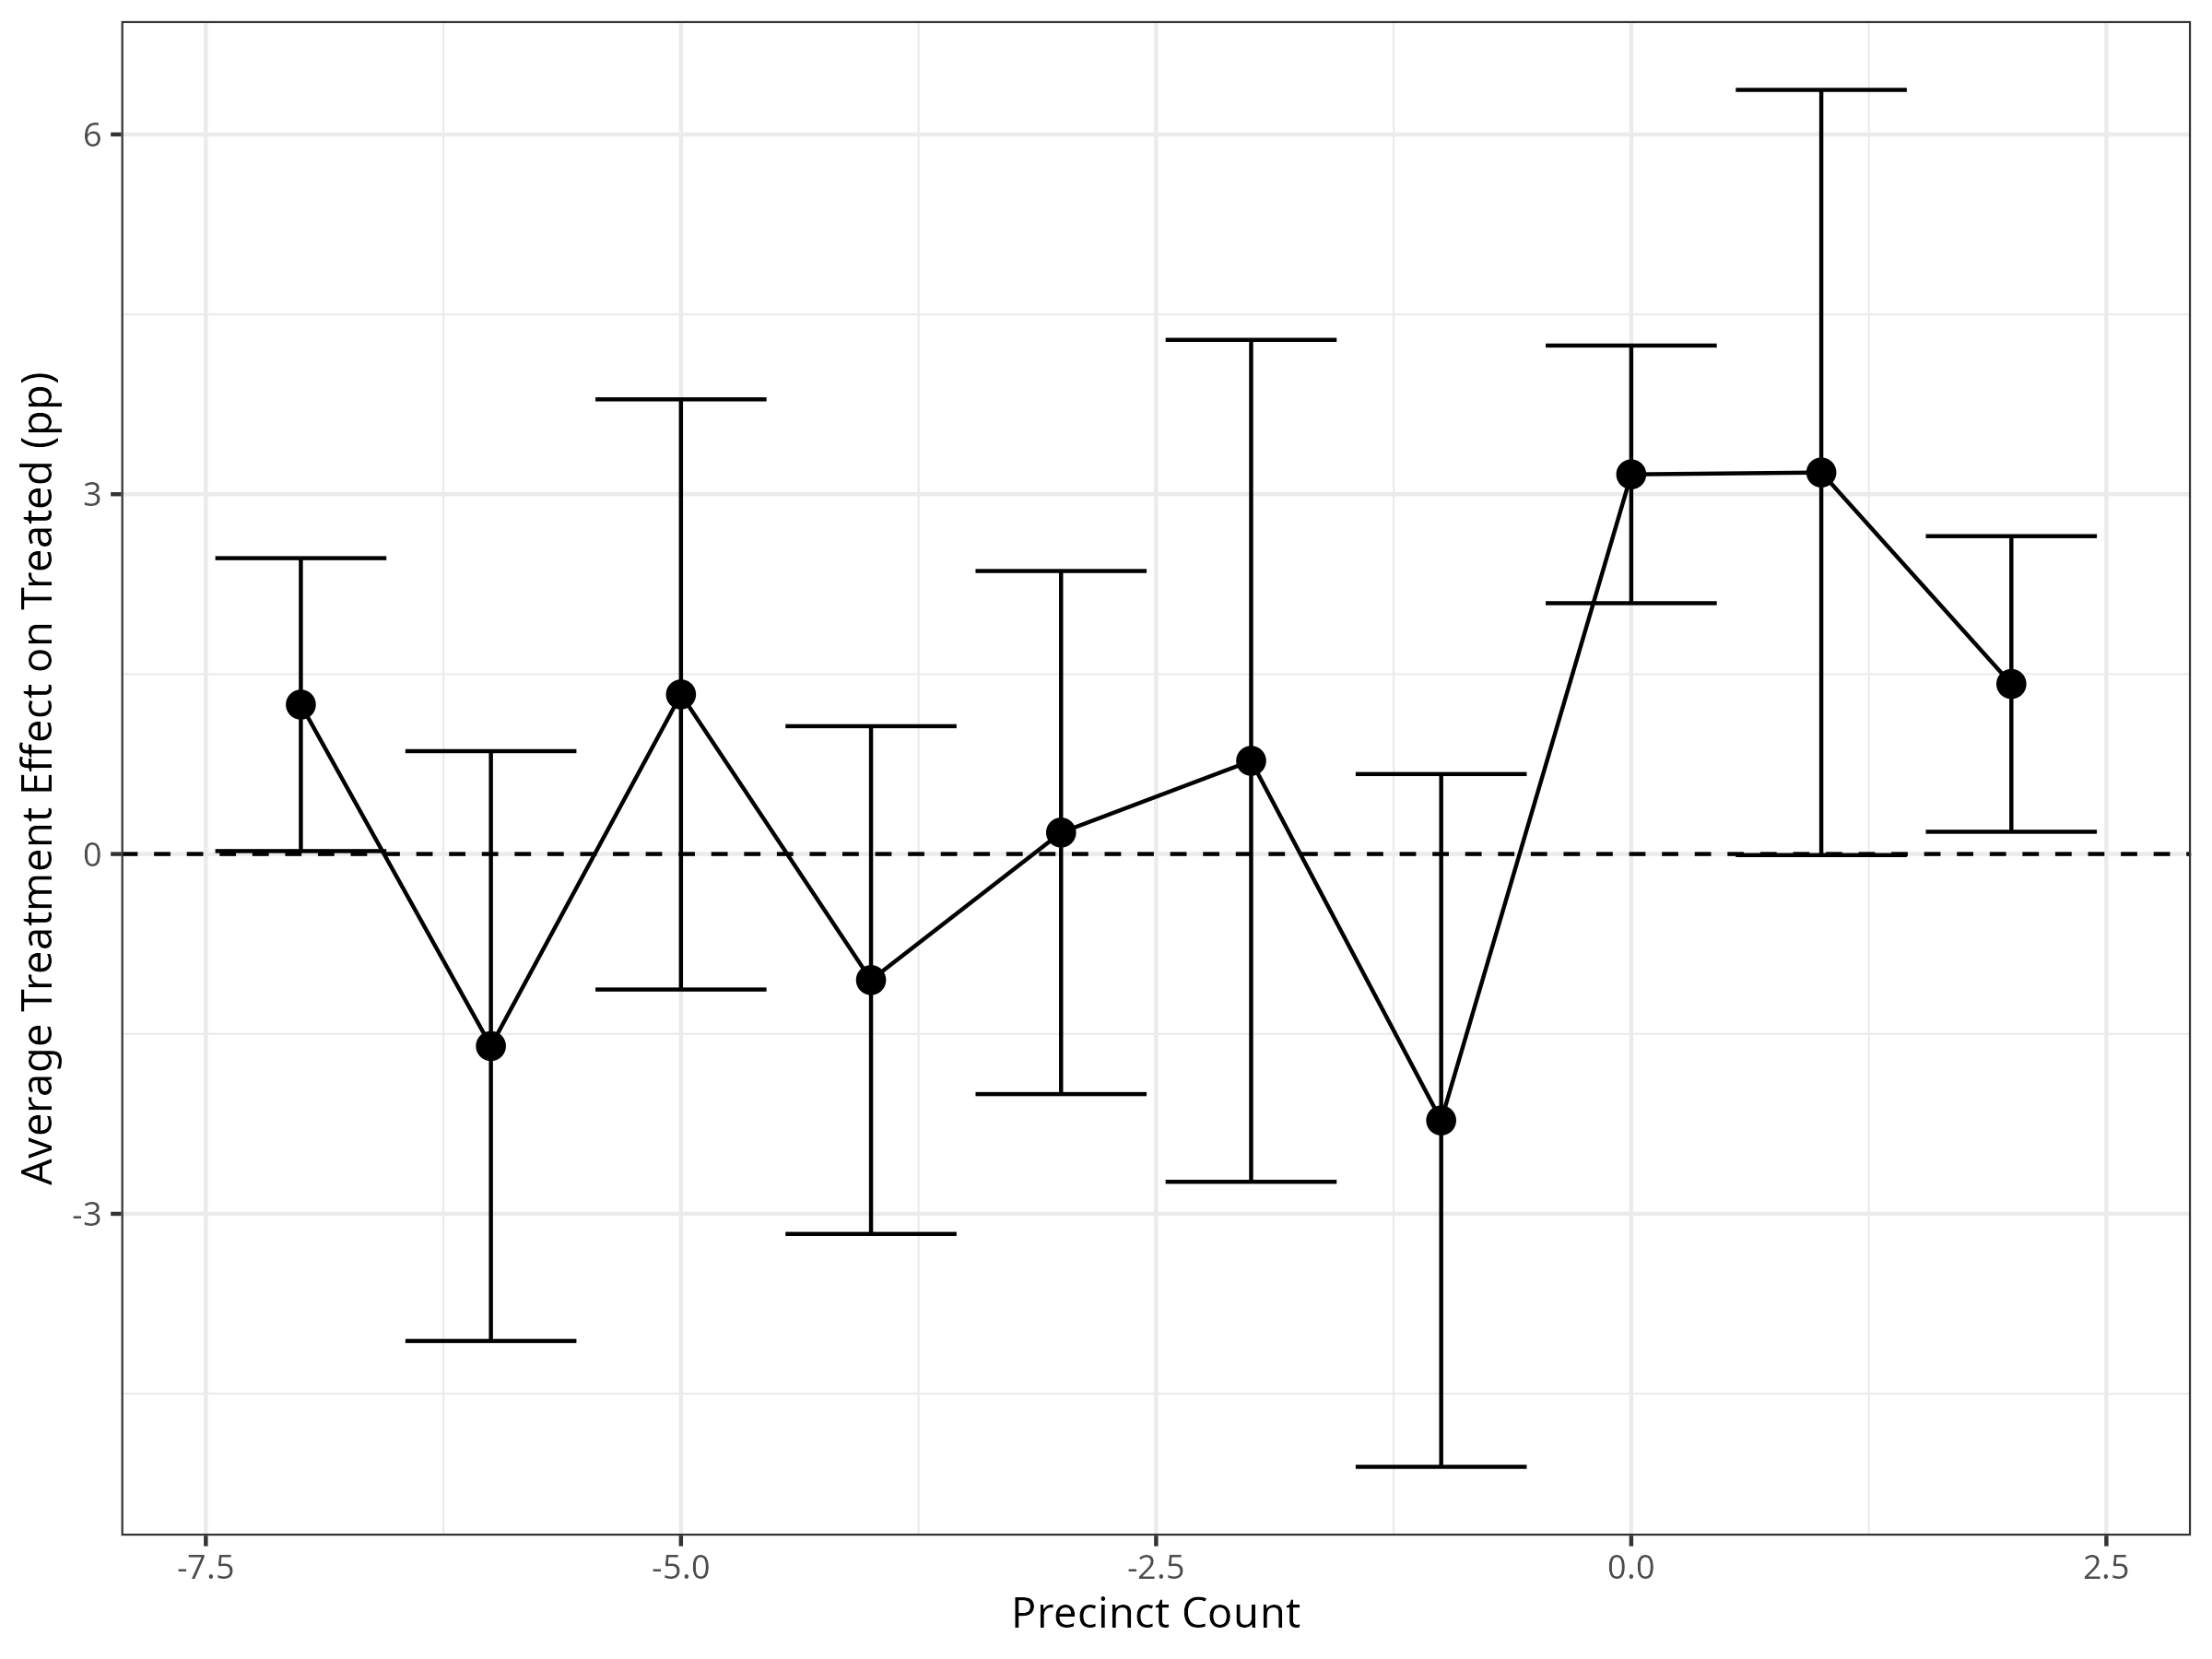
\includegraphics[width=\linewidth]{input/corrupt_8_bottom_over_time.png}
        \caption{Corruption: least supporting precincts}
        \label{fig:ATT_over_time:corruption_top}
    \end{subfigure}
\end{figure}

Lastly, the high standard errors beg the question of how stable the estimates are to the specification used.
The specifications above use the top or bottom supporting quintile, which is eight precincts, as the 2012-2022 period has an average of 41.38 precincts. 
What happens when this number is varied?
Figure~\ref{fig:ATT_across_precincts} shows the estimated ATTs for different numbers of precincts. 
The answer is that the estimates for the least supporting precincts are relatively stable in magnitude but are only statistically significant for precincts 3-8.
Most supporting precincts seem much more stable, as they are statistically significant for precincts 8-12. 

\begin{figure}[H]
    \centering
    \caption{ATT across number of precincts used}
    \label{fig:ATT_across_precincts}

    % First row
    \begin{subfigure}{.48\linewidth}
        \centering
        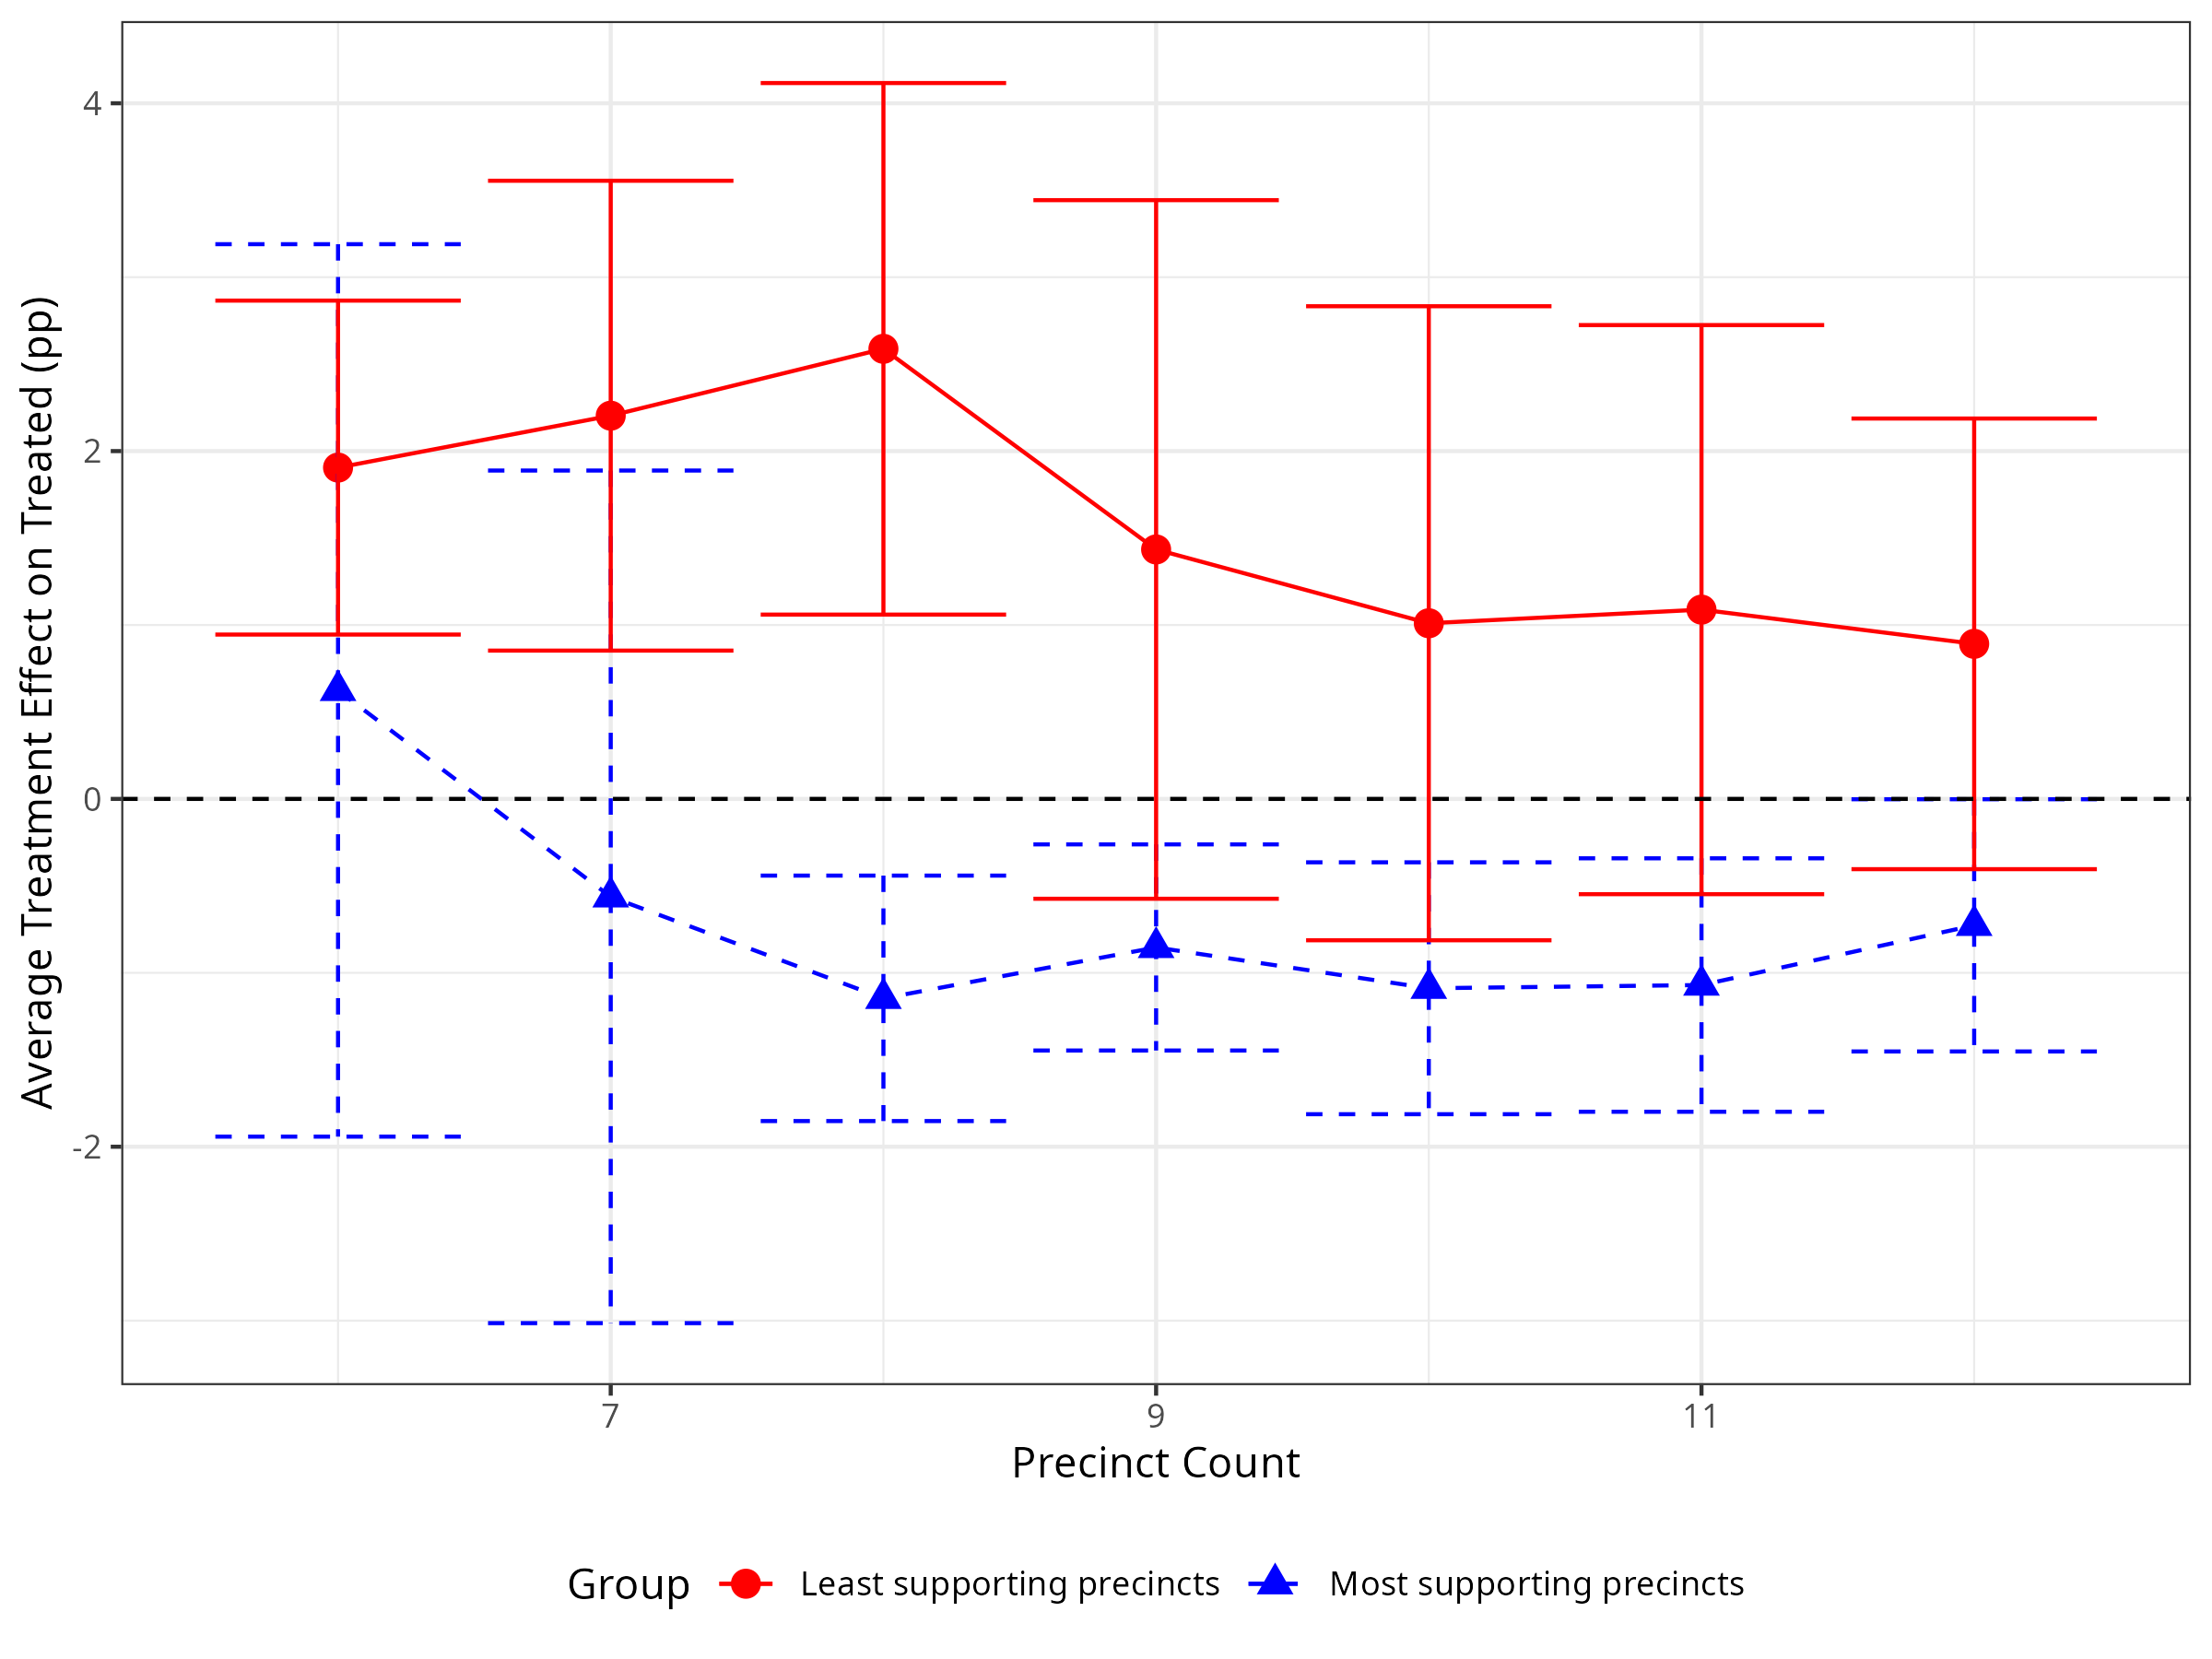
\includegraphics[width=\linewidth]{input/corruption_precinct_variation.png}
        \caption{Corruption}
        \label{fig:ATT_over_time:corruption}
    \end{subfigure}\hfill
    \begin{subfigure}{.48\linewidth}
        \centering
        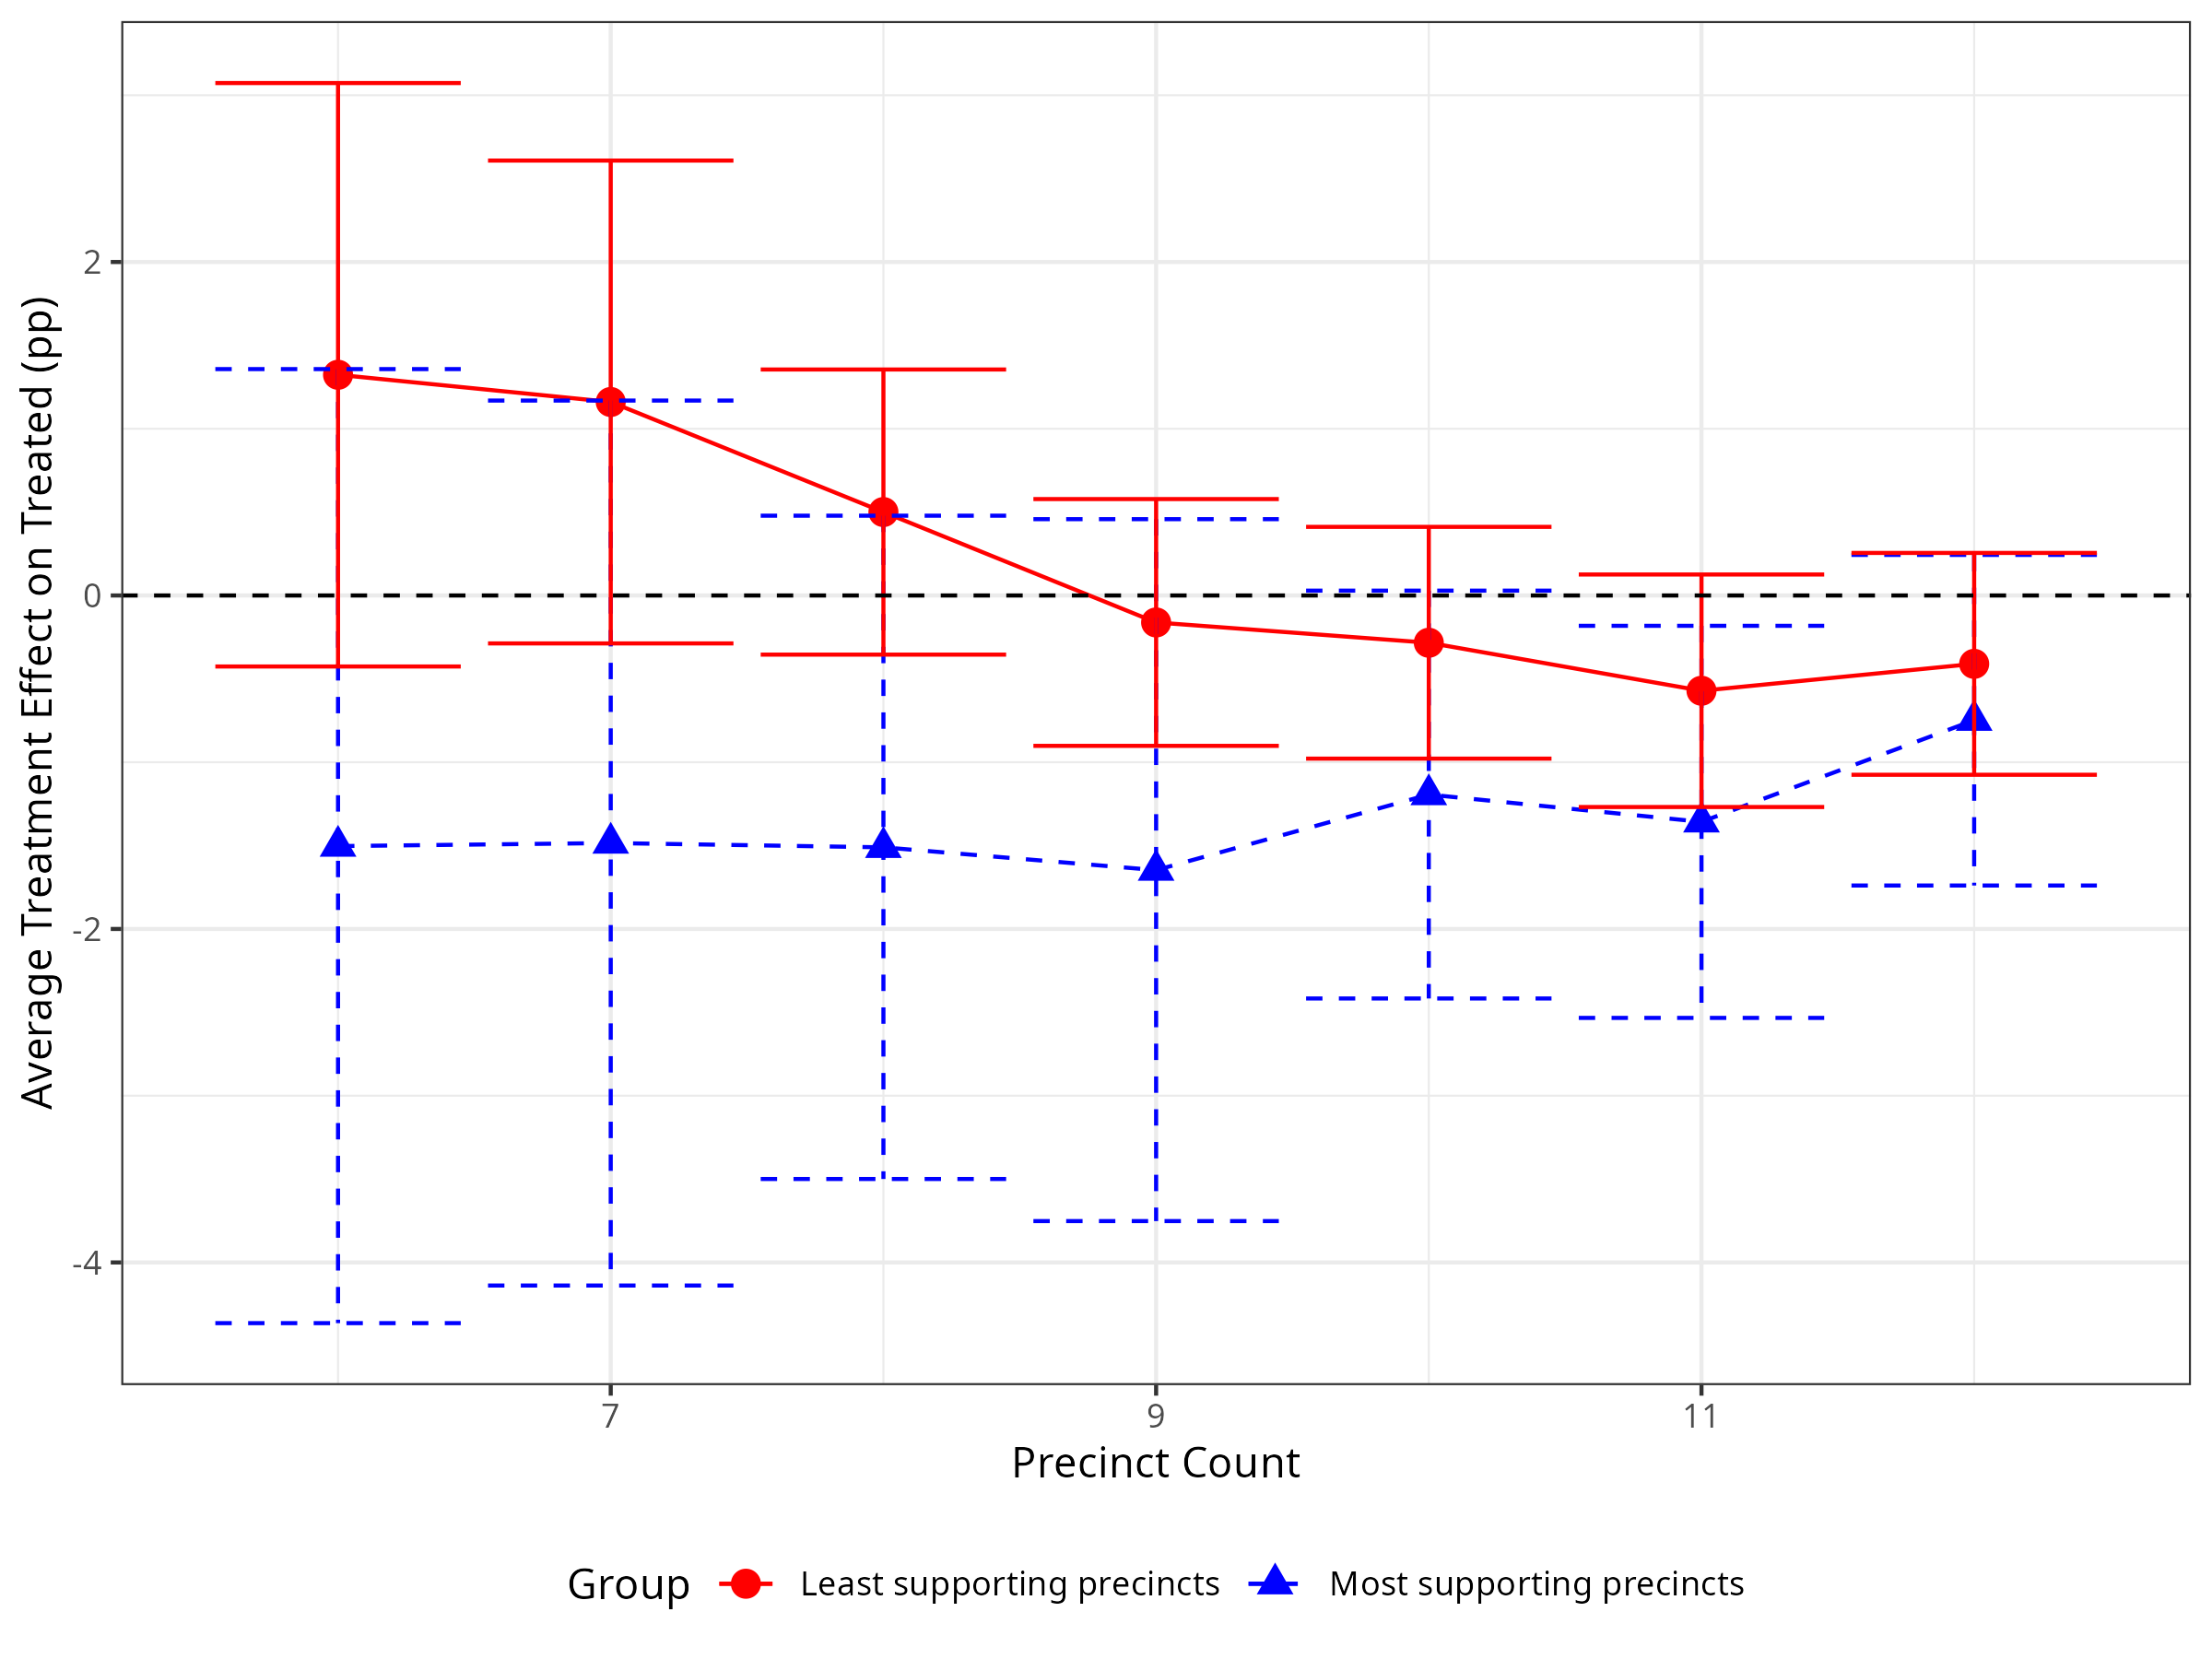
\includegraphics[width=\linewidth]{input/close_elections_precinct_variation.png}
        \caption{Close Election}
        \label{fig:ATT_across_precincts:close_election}
    \end{subfigure}
\end{figure}